\section{Front-end}

\subsection{Expanding on the Parser Monand}

\frame{
    \frametitle{Goals}
    \framesubtitle{Overview}
    \begin{itemize}
    \item Expanding on the Parser Monad
    \item Creating a front-end for the MC compiler
    \item Type-checking and normalizing
    \end{itemize}
}

\frame{
    \frametitle{What is a parser monad?}
    A parser monad iterates over a list and builds a output structure.

    If the parser fails then instead of the context it will return an error.
}

\frame{
    \frametitle{concat}
    \begin{multicols*}{3}
    \begin{enumerate}
    \item t \item w \item o \item \# \item w \item o \item r \item d \item s \item \#
    \end{enumerate}
    \columnbreak
    ch = get-char
    concat ch
    \columnbreak
    \begin{enumerate}
    \item two\#words\#
    \end{enumerate}
    \end{multicols*}
}
\frame{
    \frametitle{check char}
    \begin{multicols*}{3}
    \begin{enumerate}
    \item t \item w \item o \item \# \item w \item o \item r \item d \item s \item \#
    \end{enumerate}
    \columnbreak
    check-char \#
    \columnbreak
    \begin{enumerate}
    \item nope \item nope \item nope \item yep \item nope \item nope \item nope \item nope \item nope \item yep
    \end{enumerate}
    \end{multicols*}
}
\frame{
    \frametitle{until}
    \begin{multicols*}{3}
    \begin{enumerate}
    \item t \item w \item o \item \# \item w \item o \item r \item d \item s \item \#
    \end{enumerate}
    \columnbreak
    ch = get-char until check-char \#

    concat ch
    \columnbreak
    \begin{enumerate}
    \item two \item words
    \end{enumerate}
    \end{multicols*}
}

\frame{
    \frametitle{How to improve on it?}
    You can not really improve the parser monad itself however you can create new parser combinators.

    \begin{itemize}
    \item To manipulate the list and the context of the parser monad.
    \item To make the parser repeat until a requirement is for filled.
    \item To Manipulate the error system inside the parser monad.
    \end{itemize}

    Something that can also be improved is the error system that the parser monad uses.
}

\frame{
    \frametitle{Error handling within the parser monad}
    \begin{multicols*}{3}

    Concat all the errors
    \begin{enumerate}
    \item Slow
    \item Get all the errors and thus none
    \end{enumerate}

    \columnbreak

    Give only the last viable error
    \begin{enumerate}
    \item Fast
    \item possibility to lose error information
    \item possibility to get incorrect error information
    \end{enumerate}

    \columnbreak

    Priority for errors
    \begin{enumerate}
    \item Fast
    \item More accurate error information
    \item possibility to get incorrect error information
    \end{enumerate}
    \end{multicols*}
}

\frame{
    \frametitle{Errors with priority}
    The error with the highest priority is the one that gets returned.
    \begin{figure}
        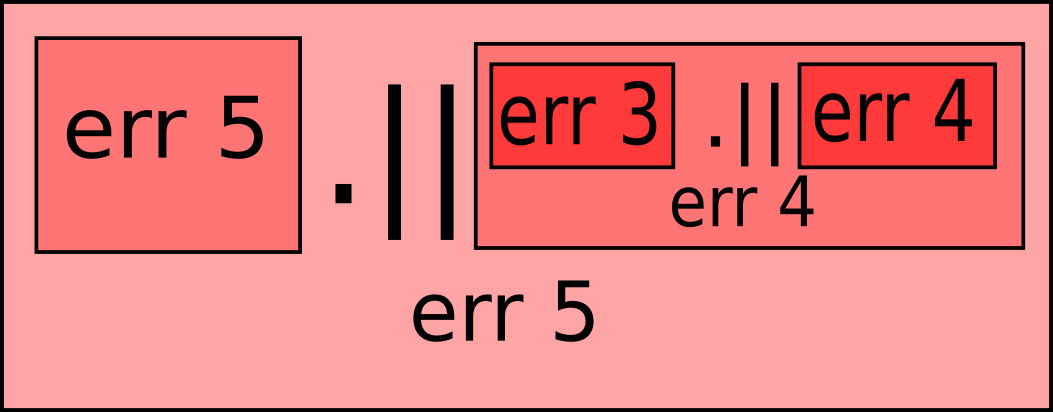
\includegraphics{error_example}
    \end{figure}
}

\subsection{Creating a front-end for the MC compiler}

\frame{
    \frametitle{Front-end}
    The front-end takes the source files and converts the code inside into an AST that can be type-checked and then used by the back-end.

}

\frame{
    \frametitle{Moving functionality from the type-checker to the parser}

    The parser monad allows for more features in the parser.

    \begin{enumerate}
    \item More detailed syntax tree
    \item Semi type-checking
    \end{enumerate}

}

\begin{frame}[fragile]
    \frametitle{Identification of function names}

    Because all function have a declaration we can generate parsers specifically made to parse this one function definition.
    \begin{lstlisting}
    Func 'a -> "add" -> 'b -> Tuple <'a 'b>
    \end{lstlisting}

    \begin{lstlisting}
    let definition_parser (decl) =
      Prs{
          let! larg = parse_left_arg decl.larg
          let! name = check_string decl.name
          let! rarg = parse_right_arg decl.rarg
          let ret = decl.ret
      }
    \end{lstlisting}
\end{frame}

\frame{
    \frametitle{Identification of variable kinds}
    Incorporating kind information in the syntax.

    \begin{itemize}
    \item Incorporating kind information in the syntax.
    \item Type has an apostrophe before its variable name. Example (`a, `generic, `type-variable)

    \item Kind has a hash before its variable name. Example (\#kind, \#module, \#term, \#type)
    \end{itemize}
}


\begin{frame}[fragile]
    \frametitle{Detection of partial application}
    The parser knows all the arguments of a function and can thus see when arguments are missing.
    A symbol table can be generated for all the variables used inside the rule.

    \begin{lstlisting}
    Func "add" -> int -> int -> int
    Func "foo" -> int -> int -> int

    add -> a0
    a0 x -> a1
    a1 y -> res
    -------------
    foo x y -> res
    \end{lstlisting}

    Symbol table.
    \begin{lstlisting}
    a0 = int -> int -> int
    a1 = int -> int
    res = int
    \end{lstlisting}
\end{frame}

\subsection{Normalizing and Type-checking}
\frame{
    \frametitle{Normalizing before type-checking}
    Because of the more precise syntax tree that the parser generates we can start the normalization procces sooner.
    Normalizing before type-checking also means that the type-checker can be further simplified.
}

\frame{
    \frametitle{Normalization}
    During normalization the premises get expanded to premises with a single instruction.
}

\begin{frame}[fragile]
    \frametitle{Normalization of data matching}
    Here we have a function with a data constructor and deconstructor.
    \begin{lstlisting}
    foo x::xs -> x,xs
    \end{lstlisting}
    During normalization the deconstructor that the rule matches on gets moved to the premises.
    And the constructor in the result also gets moved to the premises.
    \begin{lstlisting}
    _tmp0 -> x::xs
    x,xs  -> _tmp1
    ------------------
    foo _tmp0 -> _tmp1
    \end{lstlisting}
\end{frame}

\begin{frame}[fragile]
    \frametitle{Single instructures}
    When multiple expresions are in the same sentence type-checking can become complex.
    \begin{lstlisting}
        add (sub (mul 1 x) 2) 3 -> res
        -------------------------------
        foo x -> res
    \end{lstlisting}
    However if you split the sentance into multiple parts.
    \begin{lstlisting}
        mul 1 x -> _tmp0
        sub _tmp0 2 -> _tmp1
        add _tmp1 3 -> res
        --------------------
        foo x -> res
    \end{lstlisting}
    Now that the sentance is simplefied into multiple applications the complexety is moved from analyzing type signatures to building a symbol table.
\end{frame}

\begin{frame}[fragile]
    \frametitle{Type signature}
    If you write the complete signature of the sentance you will get this.
    \begin{lstlisting}
    add (sub (mul 1 x) 2) 3 -> res
    ------------------------------
    foo x -> res
    \end{lstlisting}
    \begin{lstlisting}
int -> int -> int (int -> int -> int (
    int -> int -> int int int) int) int
---------------------------------------
int -> int
    \end{lstlisting}
\end{frame}

\begin{frame}[fragile]
    \frametitle{Type signature}
    However with the normalized version you get this.
    \begin{lstlisting}
        mul 1 x -> _tmp0
        sub _tmp0 2 -> _tmp1
        add _tmp1 3 -> res
        -------------------
        foo x -> res
    \end{lstlisting}
    \begin{lstlisting}
        int -> int -> int
        int -> int -> int
        int -> int -> int
        -----------------
        int -> int
    \end{lstlisting}
    Simpler to check because now all the types are bound to a variable name and we can just iterate over the premises.
    \begin{lstlisting}
        x     = int | _tmp0 = int
        _tmp1 = int | res   = int
    \end{lstlisting}
\end{frame}
